\subsection{Wielogłowicowa głęboka rekurencyjna sieć neuronowa}
Ideą rekurencyjnych sieci neuronowych (w skrócie RNN) jest wykorzystanie dancyh w postaci sekwencji. 
Sieć neuronowa typu feed forward przyjmuje za każdym razem stałą ilość danych wejściowych i na ich podstawie generuje wynik. 
Rekurencyjna sieć neuronowa natomiast, nie konsumuje wszystkich danych wejściwych na raz. Zamiast tego,
dane pobierane są w krokach czasowych. W każdym kroku RNN wykonuje obliczenia i zwraca wyjście. 
To wyjście jest w następnym kroku łączone z jego wejściem by zwrócić kolejne dane wyjściowe. 
Ten proces jest powtarzany dopóki model nie jest wyuczony. Możliwość korzystania z 
informacji kontekstowych z poprzednich danych wejściowych jest szczególną cechą sieci typu RNN. Dlatego
są one używane do problemów gdzie kluczem do rozwiązania jest sekwencyjność danych, na przykład
przy analizie tekstów ale także sygnałów audio czy ruchów obiektów.

\begin{figure}[!ht]
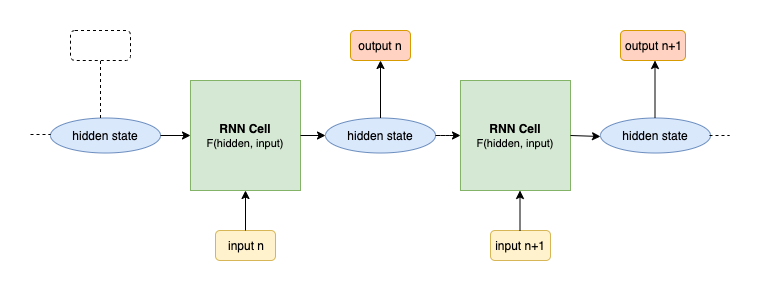
\includegraphics[width=\linewidth]{./images/rnn.png}
\caption{schemat sieci typu RNN}
\label{fig:test3}
\end{figure}
Jak widać na załączonej grafice, obliczenia dla każdego kroku czasowego są wykonywne z nowymi danymi wejściowymi
ale biorac pod uwagę kontekst z poprzedniego kroku czasowego. 
\begin{wrapfigure}{r}{0.17\textwidth}
\vspace{-4mm}
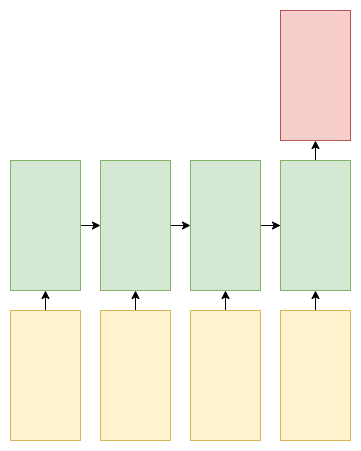
\includegraphics[width=\linewidth]{./images/many-to-one.png}
\caption{sieć typu many to one}
\label{fig:test3}
\vspace{-4mm}
\end{wrapfigure}
Rnn cell jest dokładnie tą samą przez cały proces
uczenia się. Neurony z połączeniami rekurencyjnymi działają jak pamięć - potencjalnie są w stanie modelować relacje
występujące z dowolnie długim odstępem czasowym. 
Rozwinięta w czasie sieć tworzy głęboką sieć neuronową 
ze wszystkimi tego konsekwencjami jak zanikający lub znacznie rzadziej wybuchający gradient. 
Ważną cechą tych sieci jest również fakt, że obliczenia dla długich sekwencji są bardzo kosztowne.
Sieci typu RNN generują bardzo dużo danych wyjściowych w procesie uczenia i to od nas zależy jak je 
wykorzystamy. Dla naszego problemu korzystamy z sieci typu ``many to ones'' co oznacza, że korzystamy
ze danych wyjściowych z ostatniego kroku czasowego.

Rekurencyjną sieć neuronową definiujemy jako:

\begin{align}
  &h_t = f_h(x_t, h_{t-1}) = \theta_o_h(W^Th_{t-1} + U^Tx_t) \\ 
  &y_t = f_o(h_t) = \theta_o(V^Th_t)
\end{align}

gdzie: \newline
$f_h$ - funkcja aktywacji $tanh$, \newline
$f_o$ - funkcja aktywacji $logSoftMax$, \newline
$h_t$ - warstwa ukryta w czasie $t$, \newline
$y_t$ - wektor wynikowy w czasie $t$ , \newline
$x_t$ - wektor wejściowy w czasie $t$, \newline
$W, U, V$ - macierze wag, \newline
$\theta_o, \theta_h$ - elementarne funkcje nieliniowe \newline


\begin{figure}[H]
\centering
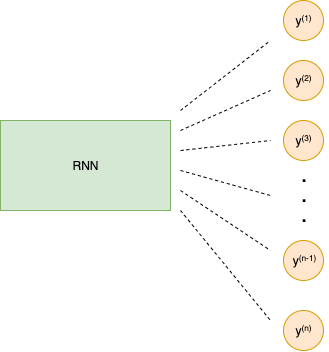
\includegraphics[height=7cm]{./images/multiheaded-rnn.png}
\caption{schemat wielogłowicowej sieci typu RNN}
\label{fig:test5}
\end{figure}

Termin ``wielogłowicowa'' odnosi się do wielu warstw liniowych które na podstawie danych wyjściowych z 
sieci rekurencyjnej predykują rozkład prawdopodobieństwa następnego znaku. Każdy autor ma swoją głowice, która 
szkolona jest tylko na jego tekstach.



